%%%%%%%%%%%%%%%%%%%%%%%%%%%%%%%%%%%%%%%%%%%%%%%%%%%%%%%%%%%%%%%%%%%%%%
%%  Copyright by Wenliang Du.                                       %%
%%  This work is licensed under the Creative Commons                %%
%%  Attribution-NonCommercial-ShareAlike 4.0 International License. %%
%%  To view a copy of this license, visit                           %%
%%  http://creativecommons.org/licenses/by-nc-sa/4.0/.              %%
%%%%%%%%%%%%%%%%%%%%%%%%%%%%%%%%%%%%%%%%%%%%%%%%%%%%%%%%%%%%%%%%%%%%%%

\newcommand{\commonfolder}{../../common-files}

\documentclass[11pt]{article}

\usepackage[most]{tcolorbox}
\usepackage{times}
\usepackage{epsf}
\usepackage{epsfig}
\usepackage{amsmath, alltt, amssymb, xspace}
\usepackage{wrapfig}
\usepackage{fancyhdr}
\usepackage{url}
\usepackage{verbatim}
\usepackage{fancyvrb}
\usepackage{adjustbox}
\usepackage{listings}
\usepackage{color}
\usepackage{subfigure}
\usepackage{cite}
\usepackage{sidecap}
\usepackage{pifont}
\usepackage{mdframed}
\usepackage{textcomp}
\usepackage{enumitem}


% Horizontal alignment
\topmargin      -0.50in  % distance to headers
\oddsidemargin  0.0in
\evensidemargin 0.0in
\textwidth      6.5in
\textheight     8.9in 

\newcommand{\todo}[1]{
\vspace{0.1in}
\fbox{\parbox{6in}{TODO: #1}}
\vspace{0.1in}
}


\newcommand{\unix}{{\tt Unix}\xspace}
\newcommand{\linux}{{\tt Linux}\xspace}
\newcommand{\minix}{{\tt Minix}\xspace}
\newcommand{\ubuntu}{{\tt Ubuntu}\xspace}
\newcommand{\setuid}{{\tt Set-UID}\xspace}
\newcommand{\openssl} {\texttt{openssl}}


\pagestyle{fancy}
\lhead{\bfseries SEED Labs}
\chead{}
\rhead{\small \thepage}
\lfoot{}
\cfoot{}
\rfoot{}


\definecolor{dkgreen}{rgb}{0,0.6,0}
\definecolor{gray}{rgb}{0.5,0.5,0.5}
\definecolor{mauve}{rgb}{0.58,0,0.82}
\definecolor{lightgray}{gray}{0.90}


\lstset{%
  frame=none,
  language=,
  backgroundcolor=\color{lightgray},
  aboveskip=3mm,
  belowskip=3mm,
  showstringspaces=false,
%  columns=flexible,
  basicstyle={\small\ttfamily},
  numbers=none,
  numberstyle=\tiny\color{gray},
  keywordstyle=\color{blue},
  commentstyle=\color{dkgreen},
  stringstyle=\color{mauve},
  breaklines=true,
  breakatwhitespace=true,
  tabsize=3,
  columns=fullflexible,
  keepspaces=true,
  escapeinside={(*@}{@*)}
}

\newcommand{\newnote}[1]{
\vspace{0.1in}
\noindent
\fbox{\parbox{1.0\textwidth}{\textbf{Note:} #1}}
%\vspace{0.1in}
}


%% Submission
\newcommand{\seedsubmission}{You need to submit a detailed lab report, with screenshots,
to describe what you have done and what you have observed.
You also need to provide explanation
to the observations that are interesting or surprising.
Please also list the important code snippets followed by
explanation. Simply attaching code without any explanation will not
receive credits.}

%% Book
\newcommand{\seedbook}{\textit{Computer \& Internet Security: A Hands-on Approach}, 2nd
Edition, by Wenliang Du. See details at \url{https://www.handsonsecurity.net}.}

%% Videos
\newcommand{\seedisvideo}{\textit{Internet Security: A Hands-on Approach},
by Wenliang Du. See details at \url{https://www.handsonsecurity.net/video.html}.}

\newcommand{\seedcsvideo}{\textit{Computer Security: A Hands-on Approach},
by Wenliang Du. See details at \url{https://www.handsonsecurity.net/video.html}.}

%% Lab Environment
\newcommand{\seedenvironment}{This lab has been tested on our pre-built
Ubuntu 16.04 VM, which can be downloaded from the SEED website. }

\newcommand{\seedenvironmentA}{This lab has been tested on our pre-built
Ubuntu 16.04 VM, which can be downloaded from the SEED website. }

\newcommand{\seedenvironmentB}{This lab has been tested on our pre-built
Ubuntu 20.04 VM, which can be downloaded from the SEED website. }

\newcommand{\seedenvironmentAB}{This lab has been tested on our pre-built
Ubuntu 16.04 and 20.04 VMs, which can be downloaded from the SEED website. }

\newcommand{\nodependency}{Since we use containers to set up the lab environment, 
this lab does not depend too much on our SEED VM. You can do this lab
using other VMs or physical machines. }







\newcommand{\seedlabcopyright}[1]{
\vspace{0.1in}
\fbox{\parbox{6in}{\small Copyright \copyright\ {#1}\ \ by Wenliang Du.\\
      This work is licensed under a Creative Commons
      Attribution-NonCommercial-ShareAlike 4.0 International License.
      If you remix, transform, or build upon the material, 
      this copyright notice must be left intact, or reproduced in a way that is reasonable to
      the medium in which the work is being re-published.}}
\vspace{0.1in}
}







\newcommand{\miniVPN}{{\tt MiniVPN}\xspace}
\newcommand{\vpnFigs}{./Figs}

\lhead{\bfseries SEED Labs -- VPN Lab: The Container Version}


\newcommand{\hostu}{{\tt U}\xspace}
\newcommand{\hostv}{{\tt V}\xspace}


\begin{document}

\begin{center}
{\LARGE VPN Lab: The Container Version}
\end{center}

\seedlabcopyright{2020}




% *******************************************
% SECTION
% *******************************************
\section{Overview}

A Virtual Private Network (VPN) is a private network built on top of a
public network, usually the Internet. Computers inside a VPN can
communicate securely, just like if they were on a real private network that
is physically isolated from outside, even though their traffic may go
through a public network. VPN enables employees to securely access a
company's intranet while traveling; it also allows companies to expand
their private networks to places across the country and around the world.


The objective of this lab is to help students understand how 
VPN works. We focus on a specific type
of VPN (the most common type), which is built on top of the transport layer.
We will build a very simple VPN from the scratch, and use the process to 
illustrate how each piece of the VPN technology works. A real VPN 
program has two essential pieces, tunneling and encryption. This lab only 
focuses on the tunneling part, helping students understand the tunneling 
technology, so the tunnel in this lab is not encrypted. 
There is another more comprehensive VPN lab that includes the encryption part.
The lab covers the following topics:  

\begin{itemize}[noitemsep]
\item Virtual Private Network
\item The TUN/TAP virtual interface 
\item IP tunneling 
\item Routing
\end{itemize}


\paragraph{Readings and videos.}
Detailed coverage of the TUN/TAP virtual interface and how 
VPN works can be found in the following:

\begin{itemize}
\item Chapter 19 of the SEED Book, \seedbook
\item Section 8 of the SEED Lecture, \seedisvideo
\end{itemize}


\paragraph{Related lab.}
This lab only covers the tunneling part of a VPN, while 
a complete VPN also needs to protect its tunnel. 
We have a separate lab, called VPN Lab, which
is a comprehensive lab, covering both tunneling and 
the protection part. Students can work on this tunneling
lab first. After learning the PKI and TLS, 
they can then move on to the comprehensive VPN lab.


\paragraph{Lab environment.} \seedenvironmentB




\newpage
% *******************************************
% SECTION
% ******************************************* 
\section{Task 1: Network Setup }


We will create a VPN tunnel between a 
computer (client) and a gateway, allowing the computer to securely access 
a private network via the gateway. 
We need at least three machines: VPN client (also serving as Host \hostu), 
VPN server (the router/gateway), and a host in the private network (Host \hostv). 
The network setup is depicted in 
Figure~\ref{vpn:fig:labsetup}.


\begin{figure}[htb]
\begin{center}
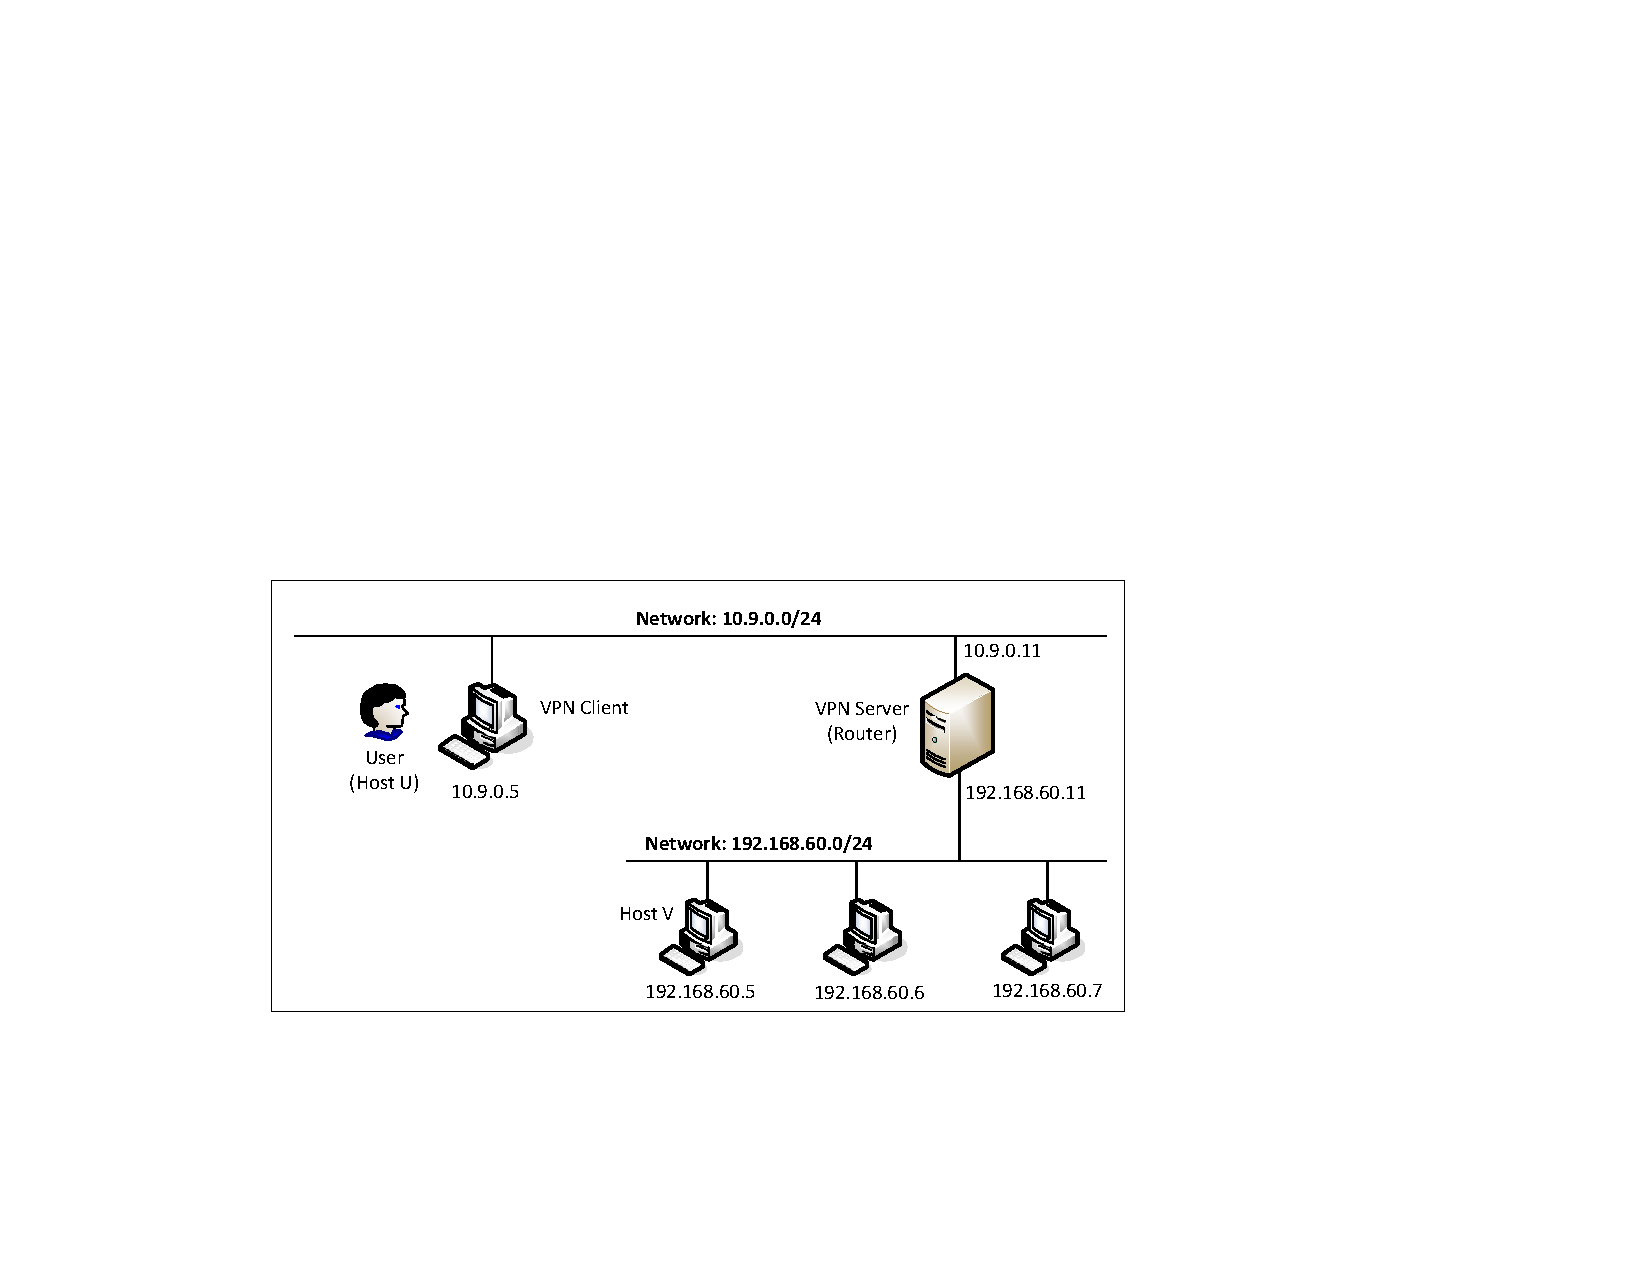
\includegraphics[width=0.9\textwidth]{./Figs/VPN_2lans.pdf}
\end{center}
\caption{Lab environment setup}
\label{vpn:fig:labsetup}
\end{figure}
 

In practice, the VPN client and VPN server are connected via the Internet.
For the sake of simplicity, we directly connect these two
machines to the same LAN in this lab, i.e., this LAN simulates the Internet. 

The third machine, Host \hostv, is a computer inside the private network. Users
on Host \hostu (outside of the private network) want to communicate with Host \hostv 
via the VPN tunnel. To simulate this setup, we connect Host \hostv to VPN Server
(also serving as a gateway).  In such a setup, 
Host \hostv is not directly accessible from the Internet; nor is it directly accessible 
from Host \hostu. 



%%%%%%%%%%%%%%%%%%%%%%%%%%%%%%%%%%%%%%%%%%%%
% Input common files related to containers

\paragraph{Container setup and commands.}



The Docker and Compose files, along with the user manual,
can be downloaded from the lab's website,
The followings Compose commands are for creating and tearing down
the lab environment. 
Since we are going to use 
these commands and several docker commands very
frequently, we have created aliases for these commands
in the \texttt{.bashrc} file.  


\begin{lstlisting}
$ docker-compose build  # Build the container image
$ docker-compose up     # Start the container
$ docker-compose down   # Shut down the container

// Aliases for commonly used docker and Compose commands. 
$ dcbuild       # Alias for: docker-compose build
$ dcup          # Alias for: docker-compose up
$ dcdown        # Alias for: docker-compose down
$ dockps        # Alias for: docker ps --format "{{.ID}}  {{.Names}}" 
$ docksh <id>   # Alias for: docker exec -it <id> /bin/bash
\end{lstlisting}



Detailed explanation of \texttt{Dockerfile} and
the \texttt{docker-compose.yml} file can be found from
the manual, which is linked to this lab's website. If you encounter
issues when setting up the lab environment, read the
``Common Problems'' section for potential solutions.


%%%%%%%%%%%%%%%%%%%%%%%%%%%%%%%%%%%%%%%%%%%%


\paragraph{Volumes.} In this lab, we need to write code and then run
the code inside containers. Code editing is more convenient inside 
the VM, so we will do it from the VM. Using the Docker \texttt{volumes},
we can create a shared folder between VM and the container. 
If you look at the \texttt{docker-compose.yml} file, you will find out that 
we have added the following entry to the VPN client and server containers.
It indicates mounting the \texttt{./volumes} folder on the host 
machine (i.e., the VM) to the \texttt{/volumes} folder inside the container.  
We will write our code in the \texttt{./volumes} folder (on the VM), so they
can be used inside the containers. 

\begin{lstlisting}
volumes:
       - ./volumes:/volumes
\end{lstlisting}
 


\paragraph{Sniffing packets.} Being able to sniffing packets is very 
important in this lab, because if things do not go as expected, being 
able to look at where packets go can help us identify the problems. 
There are two different ways to do packet sniffing:


\begin{itemize}
\item Running \texttt{tcpdump} on containers. 
We have already installed \texttt{tcpdump}
on each container. To sniff the packets going through a particular 
interface, we just need to find out the interface name, and then do the 
following (assume that the interface name is \texttt{eth0}):

\begin{lstlisting}
# tcpdump -i eth0 -n
\end{lstlisting}

It should be noted that inside containers, due to the isolation created by
Docker, when we run \texttt{tcpdump} inside a container,  
we can only sniff the packets going in and out of this container.
We won't be able to sniff the packets between other containers. 


\item Running \texttt{tcpdump} on the VM. If we run \texttt{tcpdump}
on the VM, we do not have the restriction on the containers, and
we can sniff all the packets going among containers. The interface 
name for a network is different on the VM than on the container. 
On containers, each interface name usually starts with \texttt{eth};
on the VM, the interface name for the network created 
by Docker starts with \texttt{br-}, followed by the ID of the network.  
You can always use the \texttt{ip address} command to get the 
interface name on the VM and containers. 

\item We can also run Wireshark on the VM to sniff packets.
Similar to \texttt{tcpdump}, we need to select what interface 
we want Wireshark to sniff on. 
\end{itemize}
 


\paragraph{Testing.} Please conduct the following testings to ensure that the 
lab environment is set up correctly:

\begin{itemize}[noitemsep]
\item Host \hostu can communicate with VPN Server.

\item VPN Server can communicate with Host \hostv.

\item Host \hostu should not be able to communicate with Host \hostv. 

\item Run \texttt{tcpdump} on the router, and sniff the traffic on each
of the network. Show that you can capture packets.

\end{itemize}



% *******************************************
% SECTION
% ******************************************* 
\section{Task 2: Create and Configure TUN Interface}


The VPN tunnel that we are going to build is based on the TUN/TAP 
technologies. 
TUN and TAP are virtual network kernel drivers; they 
implement network device that are supported entirely in software.
TAP (as in network tap) simulates an Ethernet device and it operates with 
layer-2 packets such as Ethernet frames; TUN (as in network TUNnel) simulates a
network layer device and it operates with layer-3 packets such as IP packets.
With TUN/TAP, we can create virtual network interfaces. 


A user-space program is usually attached to the TUN/TAP virtual network interface.
Packets sent by an operating system via a TUN/TAP network interface 
are delivered to the user-space program. On the other hand,
packets sent by the program
via a TUN/TAP network interface are injected into the operating system
network stack. To the operating system,
it appears that the packets come from an external source
through the virtual network interface.


When a program is attached to a TUN/TAP interface, IP packets sent by
the kernel to this interface will be piped into the 
program. On the other hand, IP packets written to the 
interface by the program will be piped into the kernel, as if they came from 
the outside through this virtual network interface. The program can use 
the standard {\tt read()} and {\tt write()} system calls to receive packets 
from or send packets to the virtual interface.


The objective of this task is to get familiar with the TUN/TAP technology. 
We will conduct several experiments to learn the technical details
of the TUN/TAP interface. We will use the following Python program
as the basis for the experiments, and we will modify this base 
code throughout this lab. The code is already included 
in the \texttt{volumes} folder in the zip file.  


\begin{lstlisting}[caption={Creating a TUN interface (\texttt{tun.py})}, label=vpn:list:create_tun]
#!/usr/bin/env python3

import fcntl
import struct
import os
import time
from scapy.all import *

TUNSETIFF = 0x400454ca
IFF_TUN   = 0x0001
IFF_TAP   = 0x0002
IFF_NO_PI = 0x1000

# Create the tun interface
tun = os.open("/dev/net/tun", os.O_RDWR)
ifr = struct.pack('16sH', b'tun%d', IFF_TUN | IFF_NO_PI)
ifname_bytes  = fcntl.ioctl(tun, TUNSETIFF, ifr)

# Get the interface name
ifname = ifname_bytes.decode('UTF-8')[:16].strip("\x00")
print("Interface Name: {}".format(ifname))

while True:
   time.sleep(10)
\end{lstlisting}
 


% -------------------------------------------
% SUBSECTION
% ------------------------------------------- 
\subsection{Task 2.a: Name of the Interface} 

We will run the \texttt{tun.py} program on Host \hostu.  
Make the above \texttt{tun.py} program executable, and run it using the 
root privilege. See the following commands: 

\begin{lstlisting}
// Make the Python program executable 
# chmod a+x tun.py

// Run the program using the root privilege
# tun.py
\end{lstlisting}
 

Once the program is executed, it will block. You can go to 
another terminal and get a new shell on the container. 
Then print out all the interfaces on the machine. Please 
report your observation after running the following command:

\begin{lstlisting}
# ip address
\end{lstlisting}
 

You should be able to find an interface called \texttt{tun0}. Your job 
in this task is to change the \texttt{tun.py} program, so 
instead of using \texttt{tun}  as the prefix of the interface name, use
your last name as the prefix. For example, if your last name is smith, 
you should use \texttt{smith} as the prefix.  If your last name is long,
you can use the first five characters. Please show your results. 
 


% -------------------------------------------
% SUBSECTION
% ------------------------------------------- 
\subsection{Task 2.b: Set up the TUN Interface}


At this point, the TUN interface is not usable, because it has not been configured yet. 
There are two things that we need to do before the interface can be used. First, we 
need to assign an IP address to it. Second, we need to bring up the interface, because
the interface is still in the down state. We can use the following two commands
for the configuration: 


\begin{lstlisting}
// Assign IP address to the interface 
# ip addr add 192.168.53.99/24 dev tun0

// Bring up the interface
# ip link set dev tun0 up
\end{lstlisting}
 

To make life easier, students can add the following two lines of code
to \texttt{tun.py}, so the configuration can be automatically
performed by the program. 


\begin{lstlisting}
os.system("ip addr add 192.168.53.99/24 dev {}".format(ifname)) 
os.system("ip link set dev {} up".format(ifname))              
\end{lstlisting}



After running the two commands above, run the \texttt{"ip address"} command 
again, and report your observation. How is it different from
that before running the configuration commands?



% -------------------------------------------
% SUBSECTION
% ------------------------------------------- 
\subsection{Task 2.c: Read from the TUN Interface}


In this task, we will read from the TUN interface. Whatever coming out from the TUN interface 
is an IP packet. We can cast the data received from the interface into a Scapy \texttt{IP} 
object, so we can print out each field of the IP packet. Please use the 
following \texttt{while} loop to replace the one in \texttt{tun.py}:  

\begin{lstlisting}
while True:
   # Get a packet from the tun interface
   packet = os.read(tun, 2048)
   if True:
      ip = IP(packet)
      print(ip.summary())
\end{lstlisting}


Please run the revised \texttt{tun.py} program on Host \hostu, configure the 
TUN interface accordingly, and then 
conduct the following experiments. Please 
describe your observations: 


\begin{itemize}
\item On Host \hostu, \texttt{ping} a host in the \texttt{192.168.53.0/24} network. 
What are printed out by the \texttt{tun.py} program? What has happened? Why?   

\item On Host \hostu,  \texttt{ping} a host in the internal network \texttt{192.168.60.0/24}, 
Does \texttt{tun.py} print out anything? Why?   
\end{itemize}
 



% -------------------------------------------
% SUBSECTION
% ------------------------------------------- 
\subsection{Task 2.d: Write to the TUN Interface} 


In this task, we will write to the TUN interface. Since this is a virtual network 
interface, whatever is written to the interface by the application will
appear in the kernel as an IP packet.


We will modify the \texttt{tun.py} program, so after getting a packet from the TUN interface, 
we construct a new packet based 
on the received packet. We then write the new packet to the TUN interface.
How the new packet is constructed is up to students. The code in the following
shows an example of how to write an IP packet to the TUN interface. 


\begin{lstlisting}
# Send out a spoof packet using the tun interface
newip  = IP(src='1.2.3.4', dst=ip.src)
newpkt = newip/ip.payload
os.write(tun, bytes(newpkt))
\end{lstlisting}

Please modify the \texttt{tun.py} code according to the following requirements:

\begin{itemize}
\item After getting a packet from the TUN interface, if this packet
is an ICMP echo request packet, construct a corresponding 
echo reply packet and write it to the TUN interface. Please provide
evidence to show that the code works as expected. 

\item Instead of writing an IP packet to the interface, write some arbitrary data to the 
interface, and report your observation. 
\end{itemize}
 




% *******************************************
% SECTION
% ******************************************* 
\section{Task 3: Send the IP Packet to VPN Server Through a Tunnel} 


In this task, we will put the IP packet received from the TUN interface
into the UDP payload field of a new IP packet, and send it to another computer. 
Namely, we place the original packet inside a new packet. This is called IP tunneling. 
The tunnel implementation is just standard client/server programming.
It can be built on top of TCP or UDP. In this task, we will use UDP.
Namely, we put an IP packet inside the payload field of a UDP packet. 


\paragraph{The server program \texttt{tun\_server.py}.}
We will run \texttt{tun\_server.py} program on VPN Server.
This program is just a standard UDP server program. It 
listens to port \texttt{9090} and print out whatever is 
received.  The program assumes that the data in the UDP payload 
field is an IP packet, so it 
casts the payload to a Scapy \texttt{IP} object, and print out 
the source and destination IP address of the enclosed IP packet. 


\begin{lstlisting}[caption={\texttt{tun\_server.py}}, label=vpn:list:tun_server]
#!/usr/bin/env python3

from scapy.all import *

IP_A = "0.0.0.0"
PORT = 9090

sock = socket.socket(socket.AF_INET, socket.SOCK_DGRAM)
sock.bind((IP_A, PORT))

while True:
   data, (ip, port) = sock.recvfrom(2048)
   print("{}:{} --> {}:{}".format(ip, port, IP_A, PORT))
   pkt = IP(data)
   print("   Inside: {} --> {}".format(pkt.src, pkt.dst))
\end{lstlisting}



\paragraph{Implement the client program \texttt{tun\_client.py}.}
First, we need to modify the TUN program \texttt{tun.py}. Let's rename it, and call it 
\texttt{tun\_client.py}.  Sending data to another computer using UDP
can be done using the standard socket programming. 

Replace the \texttt{while} loop in the program with the following: 
The \texttt{SERVER\_IP} and \texttt{SERVER\_PORT} should be   
replaced with the actual IP address and port number of the server program running
on VPN Server.

\begin{lstlisting}
# Create UDP socket
sock = socket.socket(socket.AF_INET, socket.SOCK_DGRAM)

while True:
   # Get a packet from the tun interface
   packet = os.read(tun, 2048)
   if True:
      # Send the packet via the tunnel
      sock.sendto(packet, (SERVER_IP, SERVER_PORT))
\end{lstlisting}




\paragraph{Testing.} 
Run the \texttt{tun\_server.py} program on VPN Server, and then
run \texttt{tun\_client.py} on Host \hostu. To test whether the 
tunnel works or not,  \texttt{ping} any IP address belonging to the \texttt{192.168.53.0/24} network.  
What is printed out on VPN Server? Why? 


Our ultimate goal is to access the hosts inside the 
private network \texttt{192.168.60.0/24} using the tunnel. Let us 
\texttt{ping} Host \hostv, and see whether the ICMP packet is
sent to VPN Server through the tunnel. If not, what are the problems?
You need to solve this problem, so the \texttt{ping} packet can
be sent through the tunnel. This is done through routing, i.e., packets going to
the \texttt{192.168.60.0/24} network should be routed to the TUN interface and 
be given to the \texttt{tun\_client.py} program.  
The following command shows how to add an entry to the routing table:


\begin{lstlisting}
# ip route add <network> dev <interface> via <router ip>
\end{lstlisting}
 

Please provide proofs to demonstrate that when you \texttt{ping}
an IP address in the \texttt{192.168.60.0/24} network, the ICMP packets 
are received by \texttt{tun\_server.py} through the tunnel. 
 



% *******************************************
% SECTION
% ******************************************* 
\section{Task 4: Set Up the VPN Server}


After \texttt{tun\_server.py} gets a packet from the 
tunnel, it needs to feed the packet to the kernel, so
the kernel can route the packet towards its final destination. 
This needs to be done through a TUN interface, just like what 
we did in Task 2. Please modify \texttt{tun\_server.py}, so it 
can do the following: 


\begin{itemize}[noitemsep]
\item Create a TUN interface and configure it.

\item Get the data from the socket interface; treat the received data 
as an IP packet.

\item Write the packet to the TUN interface.

\end{itemize}
 

Before running the modified \texttt{tun\_server.py}, we need to enable the 
IP forwarding. 
Unless specifically configured, a computer will only act as a host, 
not as a gateway. VPN Server needs to forward packets between the private network and the 
tunnel, so it needs to function as a gateway. We need to  
enable the IP forwarding for a computer to behave like a gateway. 
IP forwarding has already been enabled on the router container. 
You can see in \texttt{docker-compose.yml} that the router
container has the following entry:

\begin{lstlisting}
sysctls:
        - net.ipv4.ip_forward=1
\end{lstlisting}


 

\paragraph{Testing.} If everything is set up properly, we can \texttt{ping}
Host \hostv from Host \hostu. The ICMP echo request packets should eventually arrive at Host \hostv
through the tunnel. 
Please show your proof. 
It should be noted that although Host \hostv will respond to the ICMP packets,
the reply will not get back to Host \hostu, because we have not set up everything yet. 
Therefore, for this task, it is sufficient to
show (using Wireshark or tcpdump) that the ICMP packets have arrived at Host \hostv.





% *******************************************
% SECTION
% ******************************************* 
\section{Task 5: Handling Traffic in Both Directions}


After getting to this point, one direction of your tunnel is complete, i.e.,
we can send packets from Host \hostu to Host \hostv via the tunnel. If we look at the
Wireshark trace on Host \hostv, we can see that Host \hostv has sent out the 
response, but the packet gets dropped somewhere. This is because 
our tunnel is only one directional; we need to set up its other direction, so returning
traffic can be tunneled back to Host U.


To achieve that, our TUN client and server programs need to read data from two interfaces, 
the TUN interface and the socket interface.  
All these interfaces are represented by file descriptors, so we need to
monitor them to see whether there are data coming from them.
One way to do that is to keep polling them, and
see whether there are data on each of the interfaces. The performance of this approach is
undesirable, because the process has to keep running in an idle loop when there is no data.
Another way is to read from an interface.  By default, read is blocking, i.e., the process will
be suspended if there are no data. When data become available, the process will be unblocked,
and its execution will continue. This way, it does not waste CPU time when there is no data.

The read-based blocking mechanism works well for one interface. If a process is waiting on
multiple interfaces, it cannot block on just one of the interfaces. It has to block on all of
them altogether.  \linux has a system call called \texttt{select()}, which
allows a program to monitor multiple file descriptors simultaneously.
To use \texttt{select()}, we need to store all the file descriptors to be monitored in a set,
and then we give the set to the \texttt{select()} system
call, which will block the process until data are available on one of the
file descriptors in the set. We can check which
file descriptor has received data. In the following Python code snippet,
we use \texttt{select()} to monitor a \texttt{TUN} and a socket file
descriptor.


\begin{lstlisting}
# We assume that sock and tun file descriptors have already been created.

while True:
  # this will block until at least one interface is ready
  ready, _, _ = select([sock, tun], [], [])

  for fd in ready:
    if fd is sock:
       data, (ip, port) = sock.recvfrom(2048)
       pkt = IP(data)
       print("From socket <==: {} --> {}".format(pkt.src, pkt.dst))
       ... (code needs to be added by students) ...

    if fd is tun:
       packet = os.read(tun, 2048)
       pkt = IP(packet)
       print("From tun    ==>: {} --> {}".format(pkt.src, pkt.dst))
       ... (code needs to be added by students) ...
\end{lstlisting}
 
Students can use the code above to replace the \texttt{while} loop
in their TUN client and server programs. The code is incomplete; students
are expected to complete it. 


\paragraph{Testing.} 
Once this is done, we should be able to communicate with Machine \hostv
from Machine \hostu, and the VPN tunnel (un-encrypted) is now complete. 
Please show your wireshark proof using about \texttt{ping} and
\texttt{telnet} commands. In your proof, you need to point out how your 
packets flow.



% *******************************************
% SECTION
% ******************************************* 
\section{Task 6:  Tunnel-Breaking Experiment}


On Host \hostu, \texttt{telnet} to Host \hostv. While keeping the
\texttt{telnet} connection alive, we break the VPN tunnel by stopping 
the \texttt{tun\_client.py} or \texttt{tun\_server.py} program.  
We then type something
in the \texttt{telnet} window. Do you see what you type? 
What happens to the TCP connection? Is the connection broken? 


Let us now reconnect the VPN tunnel (do not wait for too long). We will run the 
\texttt{tun\_client.py} and \texttt{tun\_server.py} programs again, and 
set up their TUN interfaces and routing (this is where 
you can find that including the configuration commands in the programs will
make your life much easier). Once the tunnel is re-established,
what is going to happen to the
\texttt{telnet} connection?  Please describe and explain your observations.




% *******************************************
% SECTION
% ******************************************* 
\section{Task 7: Routing Experiment on Host \hostv}

In an real VPN system, the traffic will be encrypted (this part is not covered
in this lab). That means the return traffic must come back
from the same tunnel. How to get the return traffic from Host \hostv to the VPN server
is non-trivial. Our setup simplifies the situation. In our setup, 
Host \texttt{V}'s routing table has a default setting: packets going to
any destination, except the \texttt{192.168.60.0/24} network,   
will be automatically routed to the VPN server.  

In the real world, Host \hostv may be a few hops away from the VPN server, 
and the default routing entry 
may not guarantee to route the return packet back to the VPN server. Routing tables inside a 
private network have to be set up properly to ensure that packets going to the other end of the
tunnel will be routed to the VPN server. To simulate this scenario, we will 
remove the default entry from Host \hostv, and add a more specific entry to the routing 
table, so the return packets can be routed back to the VPN server.
Students can use the following commands to remove the default entry 
and add a new entry: 

\begin{lstlisting}
// Delete the default entry
# ip route del default

// Add an entry
# ip route add <network prefix> via <router ip>
\end{lstlisting}



% *******************************************
% SECTION
% *******************************************
\section{Task 8: VPN Between Private Networks} 


\begin{figure}[htb]
\begin{center}
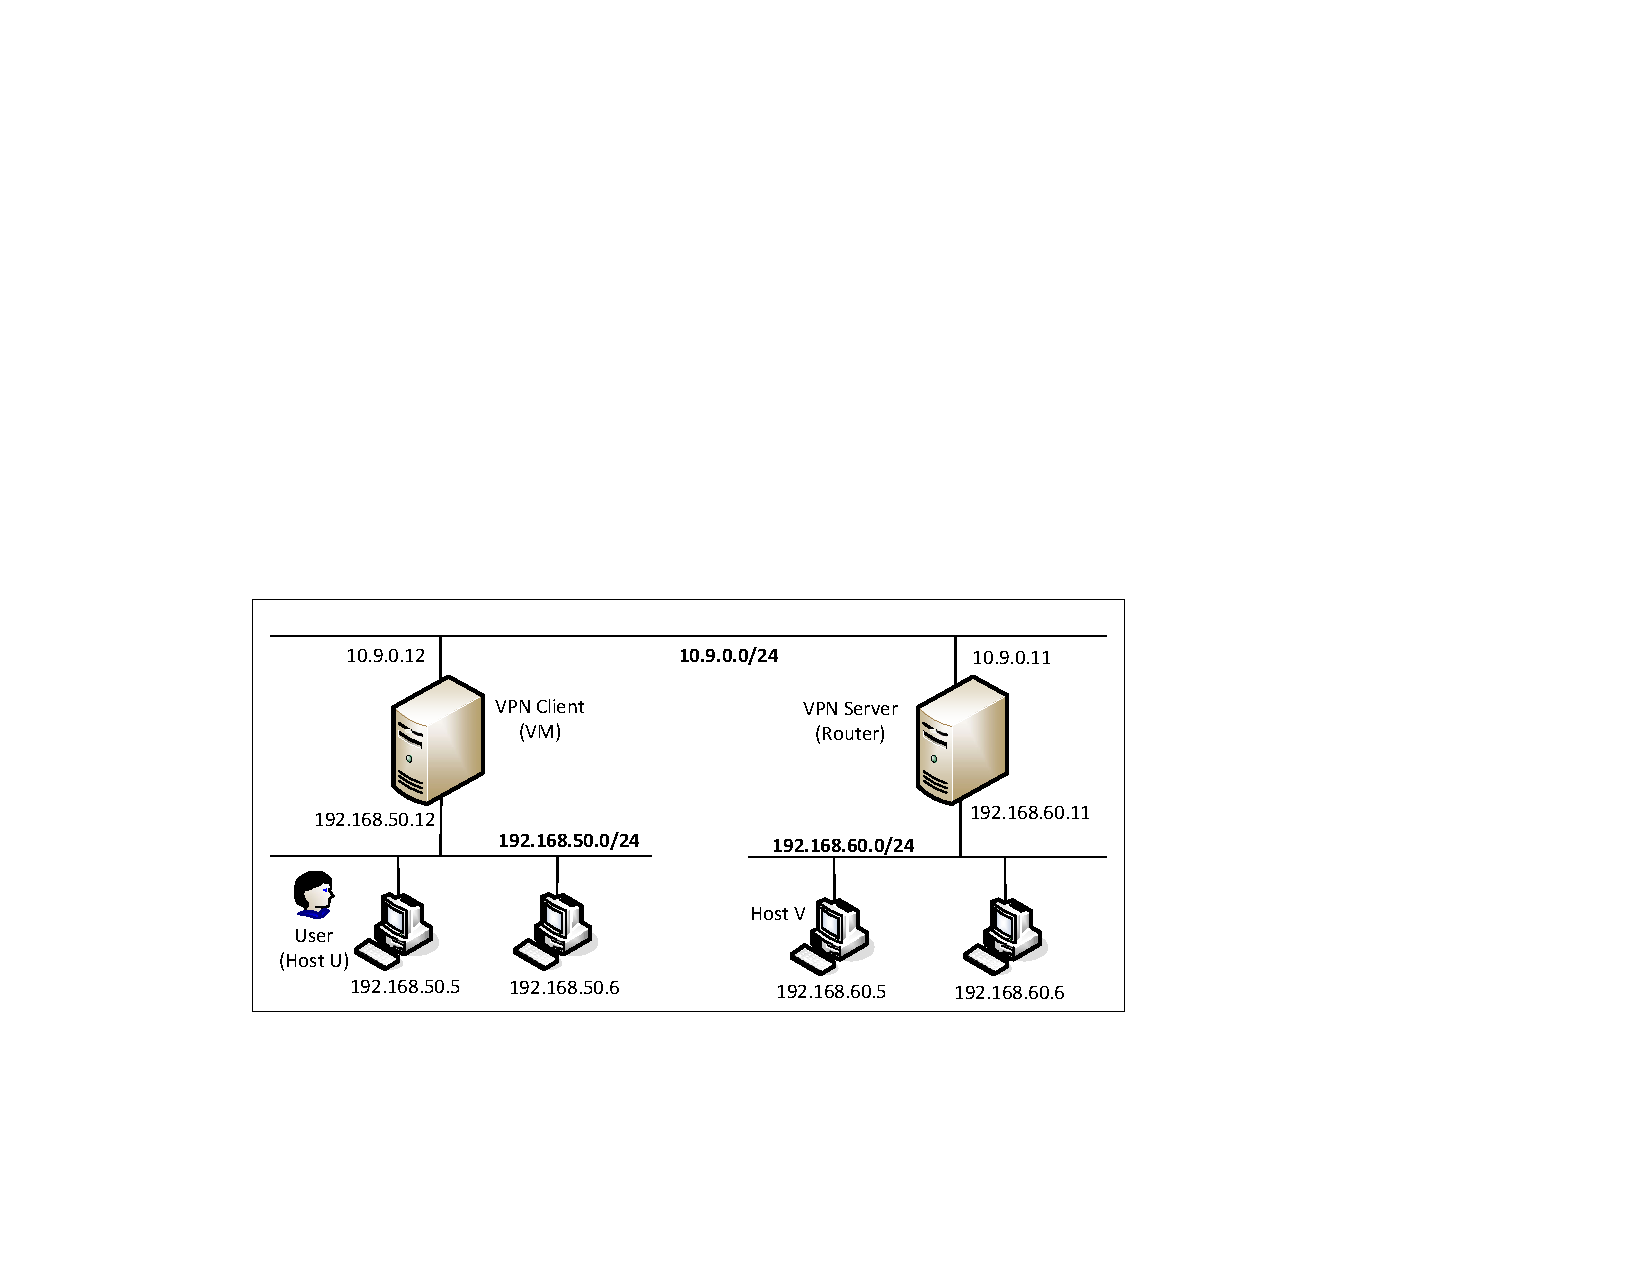
\includegraphics[width=0.8\textwidth]{Figs/VPN_3lans.pdf}
\end{center}
\caption{VPN between two private networks}
\label{vpn:fig:two-private-network}
\end{figure}
 
In this task, we are setting up a VPN between two private networks.
The setup is illustrated in Figure~\ref{vpn:fig:two-private-network}.
The whole setup is described in the \texttt{docker-compose2.yml} file, 
and you can use the \texttt{"-f docker-compose2.yml"} option to ask
\texttt{docker-compose} to use this file, instead of the 
default \texttt{docker-compose.yml} file. 


This setup simulates a situation where an organization has two sites, 
each having a private network. The only way to connect these two
networks is through the Internet. 
Your task is to set up a VPN between these two sites, so
the communication between these two networks will go 
through a VPN tunnel. You can use the code developed earlier,
but you need to think about how to set up the correct routing,
so packets between these two private networks can 
get routed into the VPN tunnel. 
In your report, please describe and explain what you did.
You need to provide proofs to show that the packets 
between the two private networks are indeed going through
a VPN tunnel. 


% *******************************************
% SECTION
% ******************************************* 
\section{Task 9: Experiment with the TAP Interface}


In this task, we will do a simple experiment with the TAP interface, so students
can get some idea of this type of interface. The way how the TAP interface works is 
quite similar to the TUN interface. The main difference is that the 
kernel end of the TUN interface is hooked to the IP layer, while the 
kernel end of the TAP interface is hooked to the MAC layer. 
Therefore, the packet going through the TAP interface includes the MAC header,
while the packet going through the TUN interface only includes the IP header. 
Other than getting the frames containing IP packets, using the TAP interface, 
applications can also get other types of frames, such as ARP frames. 


We will use the following program for our experiment, and we will
only use the VPN client container (either lab environment setup is fine).
The code 
for creating the TUN interface and TAP interface is quite similar; the 
only difference is in the interface type. For TAP interfaces, we use
\texttt{IFF\_TAP}, while for TUN,  we use \texttt{IFF\_TUN}.
The rest of the code are the same, so we do not include them in the 
following. The way to configure a TAP interface is exactly the same 
as the way to configure a TUN interface. 


\begin{lstlisting}
...

tap = os.open("/dev/net/tun", os.O_RDWR)
ifr = struct.pack('16sH', b'tap%d', (*@\textbf{IFF\_TAP}@*) | IFF_NO_PI)
ifname_bytes  = fcntl.ioctl(tap, TUNSETIFF, ifr)
ifname = ifname_bytes.decode('UTF-8')[:16].strip("\x00")
... 

while True:
   packet = os.read(tap, 2048)
   if True:
      ether = Ether(packet)
      print(ether.summary())
\end{lstlisting}
 
The code above simply reads from the TAP interface. It then casts 
the data to a Scapy \texttt{Ether} object, and prints out all 
its fields. Try to \texttt{ping} an IP address in
the \texttt{192.168.53.0/24} network; report and explain your observations.  

To make this more interesting, once you get an ethernet frame from the TAP interface,
you can check whether it is an ARP request; if it is, generate a corresponding
ARP reply and write it to the TAP interface. A sample code is provided in the
following:

\begin{lstlisting}
while True:
   packet = os.read(tun, 2048)
   if True:
      print("--------------------------------")
      ether = Ether(packet)
      print(ether.summary())

      # Send a spoofed ARP response
      FAKE_MAC   = "aa:bb:cc:dd:ee:ff"
      if ARP in ether and ether[ARP].op == 1 :
         arp       = ether[ARP]
         newether  = Ether(dst=ether.src, src=FAKE_MAC)
         newarp    = ARP(psrc=arp.pdst, hwsrc=FAKE_MAC,
                         pdst=arp.psrc, hwdst=ether.src, op=2)
         newpkt     = newether/newarp

         print("***** Fake response: {}".format(newpkt.summary()))
         os.write(tun, bytes(newpkt))
\end{lstlisting}

To test your TAP program, you can run the \texttt{arping} command
on any IP address.  This command sends out an ARP request for the specified IP address 
via the specified interface. 
If your spoof-arp-reply TAP program works, you should be able to get a 
response. See the following examples. 

\begin{lstlisting}
arping -I tap0 192.168.53.33
arping -I tap0 1.2.3.4
\end{lstlisting}

 
 
% *******************************************
% SECTION
% ******************************************* 
\section{Submission}

\seedsubmission

\end{document}







